Here is part of an op-ed essay in the New York {\em Times}: Nicholas Kristof, ``Cancer from the kitchen?'' Dec. 5, 2009.  Read it, then answer the question posed at the bottom.

\begin{quotation}

This last week I attended a fascinating symposium at Mount Sinai School of Medicine in New York, exploring whether certain common chemicals are linked to breast cancer and other ailments.

Dr. Philip Landrigan, the chairman of the department of preventive medicine at Mount Sinai, said that the risk that a 50-year-old white woman will develop breast cancer has soared to 12 percent today, from 1 percent in 1975. (Some of that is probably a result of better detection.) Younger people also seem to be developing breast cancer: This year a 10-year-old in California, Hannah, is fighting breast cancer and recording her struggle on a blog.

Likewise, asthma rates have tripled over the last 25 years, Dr. Landrigan said. Childhood leukemia is increasing by 1 percent per year. Obesity has surged. One factor may be lifestyle changes --- like less physical exercise and more stress and fast food --- but some chemicals may also play a role.

Take breast cancer. One puzzle has been that most women living in Asia have low rates of breast cancer, but ethnic Asian women born and raised in the United States don't enjoy that benefit. At the symposium, Dr. Alisan Goldfarb, a surgeon specializing in breast cancer, pointed to a chart showing breast cancer rates by ethnicity.

``If an Asian woman moves to New York, her daughters will be in this column,'' she said, pointing to ``whites.'' ``It is something to do with the environment.''

What's happening? One theory starts with the well-known fact that women with more lifetime menstrual cycles are at greater risk for breast cancer, because they're exposed to more estrogen. For example, a woman who began menstruating before 12 has a 30 percent greater risk of breast cancer than one who began at 15 or later.

It's also well established that Western women are beginning puberty earlier, and going through menopause later. Dr. Maida Galvez, a pediatrician who runs Mount Sinai's pediatric environmental health specialty unit, told the symposium that American girls in the year 1800 had their first period, on average, at about age 17. By 1900 that had dropped to 14. Now it is 12.

A number of studies, mostly in animals, have linked early puberty to exposure to pesticides, P.C.B.'s and other chemicals. One class of chemicals that creates concern --- although the evidence is not definitive --- is endocrine disruptors, which are often similar to estrogen and may fool the body into setting off hormonal changes. This used to be a fringe theory, but it is now being treated with great seriousness by the Endocrine Society, the professional association of hormone specialists in the United States.

These endocrine disruptors are found in everything from certain plastics to various cosmetics. ``There's a ton of stuff around that has estrogenic material in it,'' Dr. Goldfarb said. ``There's makeup that you rub into your skin for a youthful appearance that is really estrogen.''
\end{quotation}

Your boss has asked you to do a quick evaluation of the increase from 1 percent to 12 percent cited in the essay.  

In doing some background research, you find the following graph of age-specific {\bf invasive} breast cancer incidence rates among women 40 years old and above, from 1975 to 2003.  (Source: Jemal {\em et al.} (2007) {\em Breast Cancer Research} {\bf 9}:R28.)  

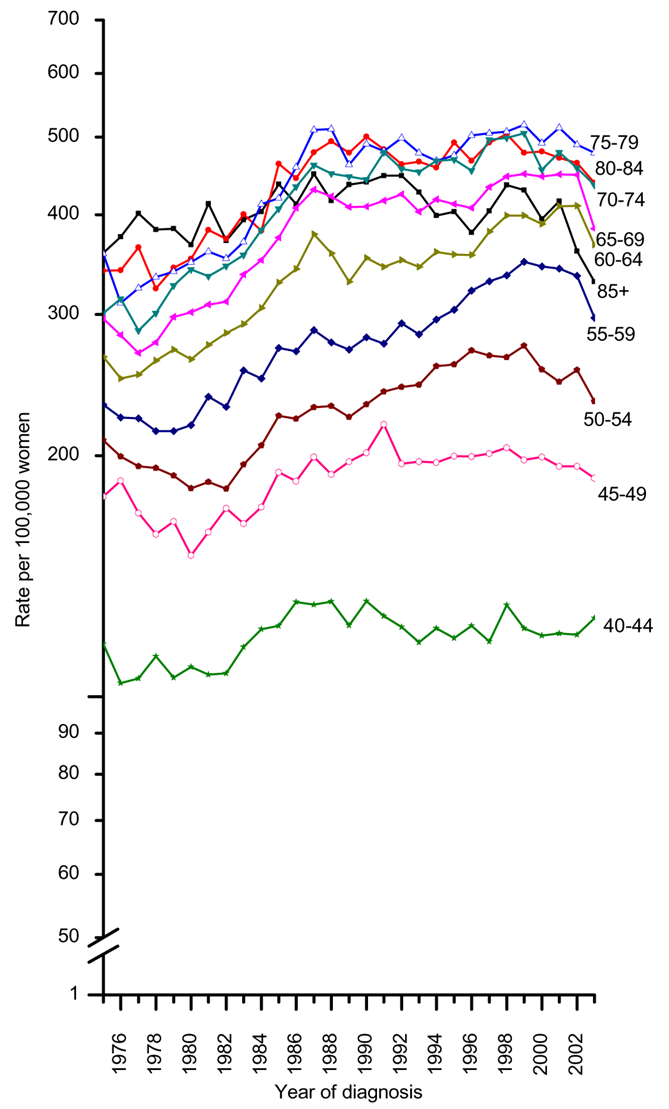
\includegraphics[width=3in]{bcr1672-1.png}

Also, with an Internet search you find that mammography started to become available in the mid 1970s, and that the current age-adjusted incidence  rate for white women is 126 per 100,000 women per year, while the death rate is 23.4 per 100,000 per year.

\begin{itemize}
\item Using this information, {\bf as well as any other knowledge you have that bears on the issue}, outline
in one or two paragraphs  what  factors other than ``common chemicals'' might account for the dramatic increase in breast cancer rates cited in the article.  

\TextEntry[itemname=dtk105-increase]

\item Describe in one or two paragraphs a reasonable design for a study to investigate the possible link between ``common chemicals'' and breast cancer.  Assume that you would need to have the study results in one or two years.  If there are serious fundamental obstacles to designing a reasonable study, say what they are.  (By ``fundamental'' obstacles, I do {\bf not} mean problems with getting funding or getting access to existing data.)

\TextEntry[itemname=dtk105-study]

\end{itemize}
